\chapter{Estado de la técnica}
\label{ch:estado_tecnica}

En este capítulo se presentan los fundamentos teóricos más relevantes que sirven como base para el desarrollo de este proyecto. Se revisan conceptos clave relacionados con el aprendizaje automático y su aplicación en la detección de \textit{malware}, así como las nociones generales de ciberseguridad y los enfoques más utilizados en la identificación de \textit{software} malicioso.

\section{Aprendizaje automático}
\label{sec:aprend_auto}

El aprendizaje automático se puede entender como <<la creación de algoritmos y modelos que permiten a los ordenadores aprender y hacer predicciones sin ser específicamente programados>> \cite{mwclass}.

\vspace{1em}

Inicialmente, los cálculos estadísticos se resolvían con máquinas electromecánicas, como la máquina tabuladora, desarrollada en 1890 por Herman Hollerith \cite{maquina_tabuladora}. Años más tarde, se presentó la neurona de McCulloch-Pitts, el primer modelo matemático de una neurona biológica, considerado por muchos como el punto de partida para el aprendizaje automático y la base de importantes modelos de cálculo \cite{inproceedings}. Hoy en día, el aprendizaje automático es esencial en diferentes ámbitos, como la investigación o los negocios, y emplea algoritmos avanzados capaces de hacer predicciones muy precisas sobre datos desconocidos.

\vspace{1em}

Los algoritmos desarrollados se pueden dividir en aprendizaje supervisado, no supervisado, semisupervisado y por refuerzo. Si nos centramos en el aprendizaje supervisado, se pueden dividir en técnicas de clasificación y regresión, siendo las primeros las que nos ocupan en este proyecto. Algunas de las principales técnicas de clasificación son: árboles de decisión, redes neuronales artificiales y máquinas de vectores de soporte (del inglés \textit{support-vector machines}, SVM).

\vspace{1em}

Todas estas técnicas se pueden adaptar a las necesidades actuales de la ciberseguridad. Los tipos de ataques, \textit{malware} o vulnerabilidades de los sistemas se están haciendo cada vez más frecuentes, no solo aumentando en cantidad, sino también en complejidad. Estos algoritmos pueden predecir si un \textit{software} es malicioso, si tiene vulnerabilidades o si un correo electrónico puede considerarse un intento de \textit{phishing}.

\vspace{1em}

A continuación se comentarán algunas de las principales técnicas de preprocesamiento, como el balanceo de datos y la reducción de la dimensionalidad, además de estudiar algunas de las métricas más comunes y modelos que podrían llegar a aplicarse en este estudio si fuera necesario.

\subsection{Balanceo de datos}
\label{subsec:balanceo}

Es muy habitual que los conjuntos de datos se encuentren desbalanceados. Esto significa que la cantidad de patrones pertenecientes a una o varias clases son significativamente menores a la clase mayoritaria. Por ejemplo, como veremos más adelante en la tabla \ref{tabla:codificacion_malware}, la clase de patrones no maliciosos representa aproximadamente la mitad del total de patrones, en torno a 150000 patrones, mientras que la clase \textit{exploit} solo tiene 12 patrones \cite{balanceo}. Debido a este desbalanceo es probable que la capacidad de generalización del modelo se vea afectada.

\vspace{1em}

Para mitigar estos problemas, las dos principales técnicas son el submuestreo y el sobremuestreo, \textit{undersampling} y \textit{oversampling} por sus términos en inglés.

\newpage
\subsubsection{Submuestreo}
\label{subsubsec:undersampling}

El \textit{undersampling} engloba las técnicas que tratan de igualar las distribuciones de datos desbalanceados eliminando muestras de las clases mayoritarias respetando la distribución de la clase minoritaria. Las soluciones a este problema pueden cambiar en función del algoritmo que decide los patrones a eliminar \cite{resamplig}. Las principales técnicas de \textit{undersampling} son:

\begin{enumerate}
	\item \textbf{\textit{Random undersampling.}} \\
		Es el método más sencillo, ya que solo se encarga de eliminar patrones de forma aleatoria de las clases mayoritarias. Lo habitual, y la técnica empleada en este estudio para la clasificación binaria, es igualar el número de patrones para cada clase. Su principal punto en contra es que puede eliminar datos útiles \cite{rundersampling}.
	\item \textbf{\textit{Condensed nearest neighbours}.} \\
		Es un algoritmo no paramétrico basado en instancias, donde la clasificación se determina a partir de los $k$ casos más cercanos al punto. Es una técnica local que utiliza medidas de distancia para identificar la similitud entre observaciones \cite{cnn}.
	\item \textbf{\textit{Tomek links.}} \\
		Consiste en identificar pares de instancias pertenecientes a clases distintas que son mutuamente los vecinos más cercanos entre sí. Suelen encontrarse en las zonas de solapamiento entre clases y representan casos ruidosos. Se elimina del conjunto de datos la instancia perteneciente a la clase mayoritaria en cada par, reduciendo así el desbalanceo \cite{tomeklinks}.
	\item \textbf{\textit{Edited nearest neighbours.}} \\
		Este método se basa en revisar cada instancia del conjunto de datos y clasificarla según la regla de los k vecinos más cercanos. Si la instancia no coincide con la clase mayoritaria de sus vecinos, se considera ruidosa o mal ubicada y se elimina del conjunto \cite{enn}.
\end{enumerate}

\subsubsection{Sobremuestreo}
\label{subsubsec:oversampling}

Las técnicas de sobremuestreo, \textit{oversampling} en inglés, buscan aumentar la representación de la clase minoritaria o de las clases minoritarias, si son más de una, generando nuevas instancias a partir de los casos existentes. El problema que presenta esta técnica es el riesgo de introducir información no real \cite{resamplig}. Entre los métodos de \textit{oversampling} más destacados se encuentran:

\begin{enumerate}
	\item \textbf{\textit{Random oversampling.}} \\
		Es la técnica más sencilla, ya que copia los patrones de la clase minoritaria o de las clases minoritarias, si hay más de una hasta alcanzar la cantidad deseada. Es habitual que se haga hasta igualar a la clase mayoritaria \cite{resamplig}.
	\item \textbf{\textit{Synthetic Minority Oversampling Technique (SMOTE).}} \\
		Genera instancias sintéticas de las clases minoritarias en lugar de replicar ejemplos existentes. Para ello, selecciona un ejemplo de la clase minoritaria y crea nuevos puntos interpolando con sus vecinos más cercanos \cite{ELREEDY201932}.
	\item \textbf{\textit{Adaptative Synthetic Sampling (ADASYN).}} \\
		Es una extensión de SMOTE que genera más instancias sintéticas en las zonas donde la clase minoritaria o de las clases minoritarias, si son más de una, es más difícil de aprender, es decir, donde está menos representada respecto a la mayoritaria \cite{ADASYN}.
\end{enumerate}

\subsection{Reducción de la dimensionalidad}
\label{subsec:red_dim}

En estadística, la reducción de la dimensionalidad es el proceso por el cual se reduce el número de variables aleatorias. Si aplicamos esto al aprendizaje automático, el objetivo a reducir es el número de características del conjunto de datos. Generalmente se aplica antes de la clasificación para evitar los efectos de la maldición de la dimensionalidad. Esta maldición implica que cuando aumenta la dimensionalidad, el volumen del espacio aumenta exponencialmente haciendo que los datos se vuelvan dispersos \cite{maldicion}.

\newpage
La principal ventaja que aportan estas técnicas es reducir el tiempo de entrenamiento y la memoria utilizada en el mismo \cite{reddim}. A continuación, estudiaremos algunos de los principales métodos.

\begin{enumerate}
	\item \textbf{Análisis de componentes principales} \\
		El análisis de componentes principales se usa para describir un conjunto de datos en términos de nuevas características no correladas, buscando la proyección donde los datos queden mejor representados según el método de mínimos cuadrados \cite{pca}.

	\item \textbf{Análisis factorial} \\
		Tiene el objetivo es identificar un conjunto reducido de factores latentes que explican la mayor parte de la varianza observada en los datos para descubrir las estructuras que generan las correlaciones entre las variables \cite{fa}.

	\item \textbf{Descomposición en valores singulares} \\
		Es una técnica algebraica que descompone una matriz en tres componentes: $U$, $\Sigma$ y $V^T$ \cite{dvs}. Esta descomposición permite representar los datos en un espacio reducido preservando la mayor parte de la información relevante.
\end{enumerate}

\subsection{Métricas de evaluación}
\label{subsec:2_metricas}

La elección de métricas de evaluación adecuadas es esencial para valorar de forma precisa el rendimiento de los modelos. No todas las métricas ofrecen la misma información. En esta sección se revisan las métricas más empleadas en la literatura especializada, destacando su utilidad, limitaciones y el tipo de información que aportan para la comparación de modelos.

\newpage
\subsubsection{Matriz de confusión}
\label{subsubsec:matrix}

Una matriz de confusión permite visualizar el rendimiento de un algoritmo de clasificación, normalmente supervisado. Cada fila representa las instancias en una clase real, mientras que cada columna representa las instancias en una clase predicha (o viceversa). La diagonal de la matriz representa las instancias correctamente clasificadas \cite{confmat}. Las matrices de confusión pueden utilizarse con cualquier algoritmo clasificador. En clasificación, las medidas suelen obtenerse de la matriz de confusión. En las Figuras \ref{fig:confmat_bin} y \ref{fig:confmat_multi} podemos ver un ejemplo para clasificación binaria y multiclase respectivamente.

\begin{figure}[H]
	\centering
	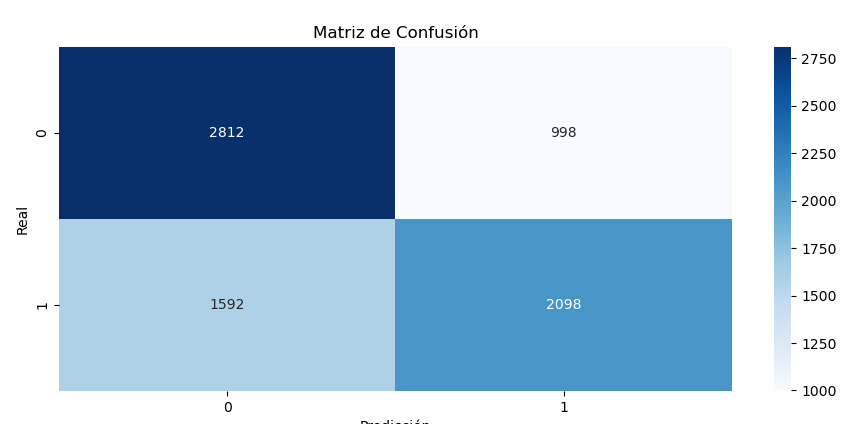
\includegraphics[width=1\linewidth]{Imagenes/confusion_binaria_ejemplo}
	\caption[Ejemplo de matriz de confusión para clasificación binaria]{Ejemplo de matriz de confusión para clasificación binaria}
	\label{fig:confmat_bin}
\end{figure}

\begin{figure}[H]
	\centering
	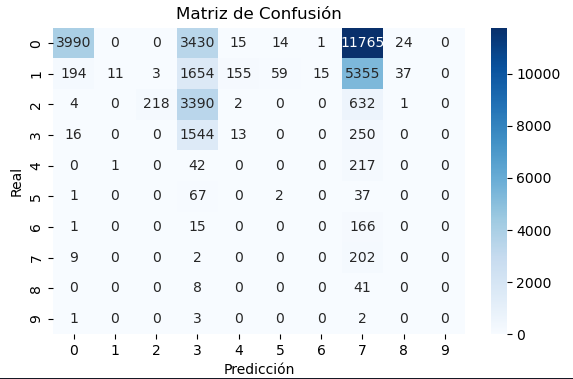
\includegraphics[width=1\linewidth]{Imagenes/confusion_multi_ejemplo}
	\caption[Ejemplo de matriz de confusión para clasificación multiclase]{Ejemplo de matriz de confusión para clasificación multiclase}
	\label{fig:confmat_multi}
\end{figure}

\subsubsection{Exactitud}
\label{subsubsec:acc}

La exactitud o \textit{Accuracy} ($CCR$) se corresponde con el porcentaje de aciertos que se han producido, es decir, los patrones clasificados correctamente respecto al total. Se calcula como la suma de verdaderos positivos ($TP$) y verdaderos negativos ($TN$) respecto al número total de patrones de entrada ($N$) \cite{metrics}.

\begin{equation}
	\label{eq:accuracy}
	\text{CCR} = \frac{TP+TN}{N}
\end{equation}

\newpage
\subsubsection{Precisión}
\label{subsubsec:prec}

La precisión es una métrica que evalúa la proporción de patrones clasificados como positivas que realmente pertenecen a la clase positiva, es decir, mide como de confiable es el modelo cuando predice un positivo. Es muy relevante cuando el coste de clasificar erróneamente un negativo como positivo es alto.

\begin{equation}
	\text{Precisión} = \frac{TP}{TP + FP}
	\label{eq:precision}
\end{equation}

Donde \(TP\) representa el número de verdaderos positivos, y \(FP\) corresponde al número de falsos positivos.

\subsubsection{Sensibilidad}
\label{subsubsec:sens}

También conocida como exhaustividad o \textit{recall} en inglés, mide la capacidad del modelo para detectar correctamente los positivos de un conjunto de datos. Como se muestra en la ecuación \ref{eq:recall}, se calcula como la proporción entre el número de verdaderos positivos ($TP$) y la suma de verdaderos positivos y falsos negativos ($FN$) \cite{metrics}. Un valor alto de sensibilidad indica que se han obtenido pocos falsos negativos.

\begin{equation}
	\label{eq:recall}
	\text{Sensibilidad} = \frac{TP}{TP + FN}
\end{equation}

\subsubsection{Mínima sensibilidad}
\label{subsubsec:ms}

La mínima sensibilidad mide cómo de bien se clasifica la clase peor clasificada. Es útil en clasificación multiclase o con conjuntos de datos desbalanceados, ya que permite identificar si existe alguna clase que el modelo no está clasificando correctamente. Un valor alto indica que el modelo mantiene un buen rendimiento en todas las clases, mientras que un valor bajo revela que, al menos, una de ellas presenta un bajo grado de acierto. Si el modelo se deja una clase sin clasificar, el valor será 0.

\vspace{1em}

Sea \( S_i \) la sensibilidad de la clase \( i \), con \( n \) el número total de clases, la mínima sensibilidad se calcula como se muestra en la ecuación \ref{eq:ms}.

\begin{equation}
	MS = \min_{i \in \{1, 2, \dots, n\}} S_i
	\label{eq:ms}
\end{equation}

Donde la sensibilidad de cada clase \( S_i \) se obtiene mediante la ecuación \ref{eq:recall}

\subsubsection{Valor-F1}
\label{subsubsec:f1}

El valor-F1 o \textit{F1-score} mide el equilibrio entre la precisión y la sensibilidad \cite{metrics}. Se calcula como la media armónica entre ambas, lo que penaliza de forma más severa los valores extremos y proporciona una medida equilibrada del rendimiento del modelo. Es especialmente útil en problemas con clases desbalanceadas, ya que evita que un alto rendimiento en una sola métrica distorsione la evaluación global. Su ecuación se describe como:

\begin{equation}
F_1 = \frac{2 \cdot TP}{2 \cdot TP + FP + FN}
\end{equation}

\subsection{Validación cruzada}
\label{subsec:validacion}

La validación es esencial en la experimentación con modelos de aprendizaje automático, ya que permite evaluar de manera fiable la capacidad de generalización del modelo, reduciendo el sesgo que podría aparecer al hacer una única partición entrenamiento/prueba.

\vspace{1em}

Se usa para para evaluar los resultados de un análisis estadístico y garantizar que son independientes de la partición entre datos de entrenamiento y prueba. Para ello hay que calcular la media aritmética obtenida de las medidas de evaluación sobre diferentes particiones. Este método es habitual cuando el objetivo es la predicción y se quiere estimar la precisión de los modelos que se van a utilizar \cite{crossval}. A continuación, se estudian las principales estrategias de validación cruzada.

\begin{enumerate}
	\item \textbf{Validación cruzada de $K$ iteraciones} \\
		Los datos en $k$ subconjuntos, usando en cada iteración uno como prueba y los restantes ($k-1$) como entrenamiento. El proceso se repite $k$ veces y los resultados se promedian para obtener una única estimación del rendimiento. Ofrece mucha precisión, pero es muy costoso computacionalmente \cite{crossval1}.
	\newpage
	\item \textbf{Validación cruzada aleatoria} \\
		En este caso se eligen aleatoriamente los datos que pertenecen a cada partición de entrenamiento y prueba. El resultado es la media aritmética de los valores obtenidos para las métricas en cada iteración \cite{crossval2}.
	\item \textbf{Validación cruzada dejando uno fuera} \\
		En este tipo de validación se separan los datos de forma que tenemos una sola muestra para los datos de prueba, mientras que para los de entrenamiento tenemos el resto de patrones del conjunto de datos. Se realizan tantas iteraciones como muestras ($N$) tenga el conjunto de datos, calculando el error para cada una de ellas como evaluación y se obtiene la media aritmética de todas ellas \cite{crossval3}.

		\[
			E = \frac{1}{N} \sum_{i=1}^{N} E_{i}
		\]
\end{enumerate}

\subsection{Algoritmos de clasificación}
\label{subsec:clasificacion}

En esta sección se presentan algunos algoritmos de clasificación más comunes, entre ellos, los que se van a usar en el estudio. Los clasificadores son modelos de aprendizaje automático capaces de asignar una etiqueta a cada instancia de datos en función de sus características. Se describen tanto modelos simples y rápidos, que facilitan la interpretación de los resultados, como modelos más complejos, que ofrecen un mayor potencial de generalización y precisión.

\subsubsection{Árboles de decisión}
\label{subsubsec:arboles}

Son modelos de aprendizaje supervisado que representan las decisiones mediante una estructura jerárquica de nodos y ramas. Cada nodo interno evalúa un atributo de los datos y realiza una bifurcación según el valor de dicho atributo, mientras que los nodos hoja asignan la clase final. Normalmente usando criterios como la ganancia de información o el índice Gini \cite{dt_ibm,dt_sklearn}.

\newpage
\paragraph*{\textbf{Ventajas.}}
\begin{itemize}
	\item La estructura del árbol es visual y fácil de entender.
	\item Una vez construido, clasificar nuevas instancias es muy rápido.
	\item Puede manejar datos categóricos y continuos sin necesidad de gran preprocesamiento.
	\item No asume ninguna distribución particular de los datos, adaptándose a distintas formas de patrones.
\end{itemize}

\paragraph*{\textbf{Inconvenientes.}}
\begin{itemize}
	\item Los árboles pueden crecer demasiado y memorizar el conjunto de entrenamiento, perdiendo capacidad de generalización.
	\item Cambios leves en los datos pueden alterar la estructura del árbol de manera significativa.
	\item Limitada capacidad predictiva para relaciones complejas.
\end{itemize}

\subsubsection{\textit{Random forest}}
\label{subsubsec:randomforest}

\textit{Random forest} es un método de ensamblado que construye múltiples árboles de decisión sobre distintas muestras del conjunto de datos y combinando aleatoriamente subconjuntos de características. Cada árbol individual realiza su predicción, y el bosque final decide por mayoría de votos (en clasificación) o promedio (en regresión). Esta estrategia reduce la varianza y mejora la capacidad de generalización respecto a un único árbol de decisión, manteniendo robustez frente al ruido y al sobreajuste \cite{rf_sklearn,rf_wiki1,rf_wiki2}.

\newpage
\paragraph*{\textbf{Ventajas.}}
\begin{itemize}
	\item Es uno de los clasificadores más certeros.
	\item Suele obtener mejores resultados que un árbol individual.
	\item Maneja variables categóricas y continuas y tolera datos faltantes.
	\item Permite identificar qué atributos contribuyen más a la predicción.
\end{itemize}

\paragraph*{\textbf{Inconvenientes.}}
\begin{itemize}
	\item Al estar compuesto por muchos árboles, es difícil interpretar.
	\item Entrenar y almacenar múltiples árboles requiere más recursos que un árbol único.
	\item Puede sobreajustar en ciertas tareas de clasificación o regresión.
\end{itemize}

%\newpage
\subsubsection{\textit{$k$-Nearest Neighbors}}
\label{subsubsec:kneighbors}

El método de los $k$ vecinos más cercanos es un método de clasificación supervisada no paramétrico que estima la probabilidad de que un patrón pertenezca a una clase. Es un tipo de aprendizaje vago, donde la función se aproxima localmente y el cálculo se hace en la clasificación \cite{knn_wiki}.

\vspace{1em}

Funciona asignando a un archivo o programa nuevo la categoría de sus vecinos más cercanos en un conjunto de datos previamente etiquetado. Es decir, compara el nuevo caso con las muestras conocidas y lo clasifica según la mayoría de etiquetas entre los más similares. La cercanía se mide normalmente usando la distancia euclidiana \cite{knn_sklearn}.

\subsubsection{\textit{Ridge}}
\label{subsubsec:ridge}

El clasificador \textit{Ridge} se basa en la regresión lineal, pero incorpora un término de penalización que evita que los coeficientes del modelo se vuelvan demasiado grandes. De esta forma, se controla el sobreajuste y se mejora la capacidad de generalización en datos nuevos. En la práctica, \textit{Ridge} busca un equilibrio entre ajustar bien los datos de entrenamiento y mantener la complejidad del modelo bajo control \cite{ridge_sklearn}.

\newpage
\subsubsection{Perceptrón multicapa}
\label{subsubsec:mlp}

Un perceptrón es el modelo matemático más simple para representar una neurona, una célula especializada que posee una cantidad indefinida de canales de entrada y un canal de salida. Los canales de entrada recogen información del entorno y la envían a la neurona, que reacciona y envía una respuesta al cerebro. La labor de las neuronas se vuelve valiosa al asociarse a otras, donde el canal de salida se asocia al canal de entrada de otra.

\vspace{1em}

Esto permite construir una red, donde la información se transmite y se procesa de manera jerárquica entre múltiples capas de neuronas. En esta red llamada perceptrón multicapa, ada neurona realiza operaciones simples, pero al combinarse en capas y mediante funciones de activación no lineales, la red es capaz de modelar relaciones complejas y patrones en los datos \cite{perceptron}.

\vspace{1em}

\subsubsection{Máquinas de vectores de soporte}
\label{subsubsec:svm}

Las Máquinas de vectores de soporte permiten optimizar los márgenes de separación entre clases y funciona muy bien en problemas de clasificación complejos. Su fortaleza reside en el uso de funciones \textit{kernel}, que permiten transformar los datos en espacios de mayor dimensión y separar clases que no son linealmente separables. En la detección de \textit{malware}, donde las fronteras entre software benigno y malicioso pueden ser difusas, esto resulta especialmente útil. El principal inconveniente es que su coste computacional puede ser elevado en conjuntos de datos grandes.

\subsubsection{\textit{Light Gradient-Boosting Machine}}
\label{subsubsec:lgbm}

El clasificador \textit{Light Gradient-Boosting Machine}, es muy eficiente en problemas de clasificación con grandes volúmenes de datos y un número elevado de características. Se basa en el método de \textit{gradient boosting}, pero introduce optimizaciones como el uso de histogramas y técnicas de reducción de memoria que lo hacen más rápido y escalable que otros métodos similares. \textit{LightGBM} ha mostrado resultados competitivos estudios recientes \cite{estudio_lgbm}.

\section{Ciberseguridad}
\label{sec:ciberseguridad}

La ciberseguridad es la protección de la infraestructura informática y la información que hay en ella, abarcando \textit{software}, \textit{hardware} y redes. Para garantizar la seguridad, es esencial combinar estrategias de prevención con métodos de protección efectivos. Las estrategias de prevención, como el uso de \textit{firewalls}, \textit{software} antivirus actualizado y educación en ciberseguridad para los usuarios, se centra en identificar y mitigar posibles amenazas antes de que ocurran.

\vspace{1em}

Por otro lado, la protección se enfoca en responder a los incidentes y minimizar sus efectos, mediante herramientas como los sistemas de detección de intrusiones. Con esto, podemos llegar a la conclusión de que el objetivo de la seguridad es minimizar los riesgos de recibir un ataque y reducir el impacto en caso recibirlo \cite{ciberseguridad_def}. En esta sección nos centraremos en la ciberseguridad \textit{software}, concretamente en los aspectos relacionados con la detección y clasificación de \textit{malware}.

\subsection{Conceptos generales}
\label{subsec:ciberseguridad_general}

La ciberseguridad constituye un pilar esencial en la sociedad digital actual, donde cada vez más actividades cotidianas, económicas y sociales dependen de sistemas informáticos y redes de comunicación. Su importancia radica en garantizar que la información y los servicios digitales sean fiables y estén protegidos frente a accesos indebidos o manipulaciones maliciosas.

\vspace{1em}

Los principales objetivos de la ciberseguridad se articulan en torno a la denominada triada CIA (\textit{Confidenciality, Integrity and Availability}, por sus siglas en inglés.) \cite{triadacia}:

\begin{itemize}
	\item \textbf{Confidencialidad}: asegura que los datos solo sean accesibles por usuarios autorizados.
	\item \textbf{Integridad}: garantiza que la información no sea alterada de forma no autorizada.
	\item \textbf{Disponibilidad}: busca que los sistemas y servicios estén siempre accesibles.
\end{itemize}

En este contexto, las organizaciones y usuarios se enfrentan a amenazas comunes como que se comentarán superficialmente por su falta de relación con el proyecto. Algunas de las amenazas más frecuentes son:

\begin{enumerate}
	\item \textbf{\textit{Phishing}}: Correos electrónicos, mensajes o enlaces fraudulentos que buscan engañar al usuario para que revele información confidencial \cite{phishing}.
	\item \textbf{\textit{Malware}}: Software malicioso que diseñado para dañar sistemas, robar información o tomar control de dispositivos. Se explicará en profundidad en la sección \ref{subsec:malware}.
	\item \textbf{Denegación de servicio}: Inundación de sistemas con tráfico para interrumpir su funcionamiento y dejar servicios inaccesibles \cite{dos}.
	\item \textbf{Robo de credenciales/fuerza bruta}: Intentos de acceder a cuentas mediante contraseñas robadas, adivinación sistemática o explotación de vulnerabilidades de autenticación.
\end{enumerate}

De todas estas opciones, el objeto de estudio de este proyecto será el \textit{malware}.

\subsection{\textit{Malware}}
\label{subsec:malware}

El \textit{software} malicioso o \textit{malware} es cualquier tipo de \textit{software} que se introduce sin el consentimiento del usuario con el objetivo de dañar o comprometer la confidencialidad, integridad o disponibilidad de la información o el sistema \cite{def_malware}. Su objetivo puede ir desde la interrupción del funcionamiento de sistemas hasta el robo de información sensible o la obtención de control remoto sobre dispositivos.

\vspace{1em}

Los primeros ejemplos de \textit{malware} surgieron en las décadas de 1970 y 1980 como experimentos de laboratorio o programas con fines demostrativos. Actualmente se ha convertido en una de las amenazas externas más relevantes debido al daño que puede llegar a causar y afectando tanto a usuarios individuales como a grandes corporaciones y entidades gubernamentales. Su relevancia se ha incrementado con la expansión de la digitalización y el uso masivo de Internet, donde ataques automatizados y campañas de \textit{malware} buscan constantemente vulnerabilidades en sistemas y redes, además de posibles descuidos de los usuarios.

\subsubsection{Tipos de \textit{Malware}}
\label{subsubsec:tipos_malware}

Podemos clasificar el \textit{malware} en diferentes categorías \cite{categoriamw} según su propósito:

\begin{itemize}
	\item \textbf{Virus}. Tienen como objetivo infectar archivos y sistemas informáticos. Se propagan cuando los usuarios comparten archivos o ejecutan programas infectados.
	\item \textbf{Gusanos}. Se propagan a través de las redes sin que tenga que intervenir el usuario.
	\item \textbf{Troyanos}. Se presentan como un \textit{software} legítimo. De esta forma intentan engañar al usuario para que lo descargue, instale y ejecute.
	\item \textbf{\textit{Adware}}. Muestra anuncios de forma intrusiva. Puede ser incrustada en una página web mediante gráficos, carteles, ventanas flotantes, o durante la instalación de algún programa al usuario, con el fin de generar lucro a sus autores.
	\item \textbf{\textit{Spyware}}. Trata de conseguir información de un equipo sin conocimiento ni consentimiento del usuario. Después transmite esta información a una entidad externa.
	\item \textbf{\textit{Ransomware}}. Conocido como secuestro de datos en español. Está diseñado para restringir el acceso a archivos o partes de un sistema y pedir un rescate para quitar la restricción.
	\item \textbf{\textit{Rootkit}}. Es un conjunto de \textit{software} que permite al atacante un acceso de privilegio a un ordenador, manteniendo presencia inicialmente oculta al control de los administradores.
	\item \textbf{\textit{Keylogger}}. Se encarga de registrar las pulsaciones que se realizan en el teclado, para memorizarlas en un fichero o enviarlas a través de Internet.
	\item \textbf{\textit{Exploit}}. Aprovecha un error o una vulnerabilidad de una aplicación o sistema para provocar un comportamiento involuntario.
	\item \textbf{\textit{Backdoor}}. Puerta trasera en español. Este tipo de \textit{software} permite un acceso no autorizado al sistema, evitando pasar por los métodos de autenticación.
\end{itemize}

\subsection{Técnicas de detección de \textit{malware}}
\label{subsec:deteccion_malware}

Ningún método de detección es infalible y los principales antivirus comerciales pueden combinar distintas técnicas en función de las necesidades. La detección basada en firmas siguen siendo el método más usado en términos absolutos porque son rápidas, eficientes y fáciles de implementar. Este método consiste en comparar archivos con una base de datos de patrones conocidos. Otros mecanismos son: la detección heurística, por comportamiento, \textit{sandbox} e inteligencia artificial \cite{antivirus}.

\vspace{1em}

Existen varias limitaciones de los métodos tradicionales frente a nuevas amenazas. Por ejemplo, para evadir la detección basada en firmas se generaba una cadena de bits única cada vez que se codificaba. Esto se denomina polimorfismo. Gracias a la heurística no era necesaria una coincidencia exacta con las firmas almacenadas, pero debido a la gran cantidad de variaciones que surgen a diario, su efectividad y la de otros mecanismos se ve comprometida \cite{limitaciones}. A continuación se estudiarán algunas de las técnicas más usadas.

\subsubsection{Detección basada en firmas}
\label{subsubsec:firmas}

La detección de intrusiones basada en firmas compara la actividad del sistema con patrones conocidos de ataques para identificar comportamientos maliciosos. El código del \textit{Malware} se compila como cualquier programa, y este código se puede cifrar para crear una firma única. Otras formas de crear una firma son sus acciones en memoria o los archivos específicos que generan en ubicaciones específicas. En los casos más modernos se comunican a través de Internet hacia direcciones IP o dominios, lo que permite a los sistemas de defensa y prevención detectarlas y alertar \cite{firmas1}.

\vspace{1em}

Las firmas habitualmente son generadas y almacenadas por los proveedores comerciales de estos servicios, como pueden ser \textit{ESTET} \cite{eset} o \textit{Bitdefender} \cite{bitdefender}, aunque algunas pueden ser abiertas o colaborativas, como es el caso de \textit{VirusTotal} \cite{virustotal}.

\newpage
\paragraph*{\textbf{Ventajas.}}
Las detección basada en firmas es un sistema muy preciso, ya que si el autor del \textit{Malware} no realiza cambios en el código, la firma no cambia y la detección es casi inmediata. Esto implica que el sistema de detección proporcione muy pocos falsos positivos \cite{firmas1}.

\vspace{1em}

\paragraph*{\textbf{Inconvenientes.}}
El principal inconveniente de la detección basada en firmas es que para poder actuar, la amenaza debe ser conocida. Esto significa que no tienen forma de detectar las amenazas de tipo \textit{zero day}, es decir, que acaban de ser descubiertas y que aún no tienen una firma \cite{zeroday}.

\noindent Como se ha comentado en las ventajas, es casi infalible si no se modifica el código del programa, pero la firma queda completamente inservible con un pequeño cambio que se introduzca \cite{firmas}.

\subsubsection{Detección heurística}
\label{subsubsec:heuristica}

En la detección de \textit{Malware}, se conoce como heurística al conjunto de técnicas que se usan para identificar aplicaciones maliciosas que no se encuentran en la base de datos de firmas \cite{heu}. Surge de la necesidad de combatir las nuevas amenazas y es uno de los pocos métodos capaces de combatir los \textit{Malware} polimórficos, que cambian su código constantemente \cite{kp_heu}

\vspace{1em}

\paragraph*{\textbf{Ventajas.}}
La principal ventaja de la detección heurística es su capacidad para identificar nuevas amenazas desconocidas. Al no depender exclusivamente de firmas previas, resulta eficaz para reconocer modificaciones de \textit{Malware} existente o ataques que todavía no han sido documentados. Esto amplía la cobertura de protección frente a amenazas emergentes \cite{fortinet_heu}.

\paragraph*{\textbf{Inconvenientes.}}
Este tipo de análisis trata de detectar el comportamiento conocido, por lo que si un programa no realiza ninguna acción conocida, es probable que no sea detectado \cite{fortinet_heu}.

\subsubsection{Detección basada en comportamiento}
\label{subsubsec:comportamiento}

Esta técnica es clave frente a amenazas que pueden evitar ser detectadas por los métodos tradicionales. Los atacantes, para evitar ser detectados, ofuscan el código, práctica que ``consiste en transformar el código fuente de un programa en una forma más compleja y difícil de comprender, sin alterar su funcionalidad'' \cite{ofuscacion}.

\vspace{1em}

La detección basada en comportamiento analiza las actividades y patrones de ejecución de programas para identificar posibles amenazas y descubrir comportamientos anómalos que puedan indicar una intrusión, incluso cuando se trata de ataques desconocidos o de tipo \textit{zero day}. Es capaz de identificar amenazas desconocidas, ya que no depende de bases de datos de firmas previas pero suele generar un mayor número de falsos positivos.

\subsubsection{Detección mediante aprendizaje automático}
\label{subsubsec:ml}

Los modelos de aprendizaje automático tienen la capacidad de extraer conocimiento a partir de grandes cantidades de información y reconocer tanto patrones complejos como inusuales. Examina entradas como registros del sistema, tráfico de red, procesos en ejecución o secuencias de instrucciones para localizar conductas anómalas. Además, pueden ajustarse de forma continua incorporando nuevas muestras, lo que incrementa su efectividad frente a variantes no identificadas \cite{s2grupo}.

\vspace{1em}

En este caso, si un atacante realiza cambios en el código, lo ofusca o es un programa no conocido, no tiene por qué engañar al modelo. Esto hace que sea uno de los métodos de detección de \textit{malware} más potentes y con proyección de futuro \cite{ml_mw}.

Durante la realización de este proyecto vamos a centrarnos en la detección de \textit{malware} mediante métodos de aprendizaje automático, concretamente de clasificación nominal.
